% =====================================================================
%  Research proposal (standalone, single-file)
%  Mask-Augmented Multimodal Animal Behaviour Recognition
%  Compile:  pdflatex research_proposal.tex   (run twice for references)
%  Or drop this single file into Overleaf.
% =====================================================================
\documentclass[11pt]{article}

\usepackage[a4paper,margin=2.4cm]{geometry}
\usepackage{iftex}
\ifPDFTeX
  \usepackage[T1]{fontenc}
  \usepackage[utf8]{inputenc}
  \IfFileExists{lmodern.sty}{\usepackage{lmodern}\usepackage{microtype}}{}
\else
  \usepackage{fontspec}
  \IfFileExists{microtype.sty}{\usepackage{microtype}}{}
\fi
\usepackage{amsmath,amssymb}
\usepackage{graphicx}
\usepackage{booktabs}
\usepackage{enumitem}
\usepackage{caption}
\usepackage[dvipsnames]{xcolor}
\usepackage{tikz}
\usetikzlibrary{positioning,fit,backgrounds,arrows.meta,calc}
\usepackage[colorlinks=true,linkcolor=NavyBlue,citecolor=NavyBlue,urlcolor=NavyBlue]{hyperref}

\setlist{nosep,leftmargin=1.4em}
\captionsetup{font=small,labelfont=bf}

\title{\textbf{Mask-Augmented Multimodal Animal Behaviour Recognition}\\[2pt]
\large Does the animal's foreground silhouette \emph{shape} help recognise behaviour,\\ where background segmentation maps did not?}
\author{Kostiantyn Boiar\\[2pt]
\small MSc thesis proposal, University of Glasgow}
\date{\today}

\begin{document}
\maketitle

\begin{abstract}
\noindent Multimodal models recognise animal behaviour from video, and sometimes from audio and pose. This project asks a narrow, untested question: does adding the animal's \emph{foreground silhouette}---its outline shape, tracked through a clip---improve behaviour recognition over video(+audio) baselines, and is any benefit concentrated in the posture- and contact-defined behaviours where shape should matter most? The motivation is a specific published result: on the MammAlps benchmark, \emph{background/scene} segmentation maps did not help recognition, while audio gave a small lift~\cite{mammalps}. The nearest mask-based works use segmentation only to \emph{remove} the background or crop a region of interest~\cite{panaf,maroon}; none treats the silhouette shape itself as a fused, positive input. The design is deliberately compute-light: every heavy encoder is frozen and its features are computed once and cached, so only a small fusion head is trained. The contribution is the answer and its analysis---per-behaviour, with inter-animal contact geometry and a background-robustness test---rather than the model wiring. A clean result is useful either way.
\end{abstract}

% ---------------------------------------------------------------------
\section{Background and motivation}
% ---------------------------------------------------------------------
Recognising what an animal is \emph{doing} from camera footage underpins both neuroscience and ecology. Recent benchmarks combine several signals. MammAlps~\cite{mammalps} is a multimodal, multi-view wildlife benchmark (video, audio, and reference segmentation maps; 11 activities and 19 actions across five species) with a VideoMAE-based baseline. Two of its findings frame this proposal. First, audio gives a small but real improvement over video alone. Second, the \emph{reference scene segmentation maps}---a single \emph{semantic map of the background} per fixed camera viewpoint, drawn from an animal-free photo and held essentially static across a clip---did \emph{not} improve over the video or video+audio models. Such a map encodes \emph{where} the camera sits (habitat, terrain, vegetation): context that correlates with species and location, but says nothing about \emph{what the animal's body is doing}; telling the model about the static background does not help it read behaviour. The distinction matters for everything that follows: MammAlps already \emph{segments}---but it segments the \emph{scene}, not the animal.

A parallel result comes from PanAf-FGBG~\cite{panaf}, which pairs each chimpanzee video with a matching empty-background video and uses SAM\,2 masks to \emph{erase} the animal and synthesise backgrounds. Its purpose is to expose how strongly models lean on behaviour-correlated background, and how that hurts out-of-distribution generalisation. Crucially, the mask there is a tool for \emph{removing} the foreground; the object of study is the background.

Pose-based pipelines (e.g. ST-GCN~\cite{stgcn} and, in the host group, PoseR~\cite{poser}) instead encode the animal's skeleton. Pose is compact and effective, but keypoints capture body \emph{configuration} only sparsely---and weakly capture two-body contact, where the relevant signal is how two bodies overlap and touch. LookAgain~\cite{lookagain} reports exactly this asymmetry: added visual context helps some contact behaviours yet not those whose geometry pose already pins down.

The gap is the obvious next question nobody has tested. If the background does not help (MammAlps) and models over-rely on it (PanAf-FGBG), what about the one representation that throws the background away entirely and keeps only the animal's shape? This is a different \emph{object} of segmentation: where MammAlps' map is a \emph{static, scene-level} segmentation of the background, ours is a \emph{per-frame foreground} (instance) segmentation of the animal itself---a silhouette whose changing outline \emph{is} posture, and whose overlap with a second animal's mask \emph{is} contact. Treating this \emph{foreground silhouette as a fused, positive modality}---rather than a background-removal tool or an ROI crop---is unaddressed.

% ---------------------------------------------------------------------
\section{Research questions and hypotheses}
% ---------------------------------------------------------------------
\begin{description}[leftmargin=2.2em,style=nextline]
  \item[RQ1 (does it help?)] Does fusing silhouette-shape features improve behaviour recognition over video and over video+audio baselines?
  \item[RQ2 (where?)] Is any improvement concentrated in posture- and contact-defined behaviours (e.g. chasing, huddling, mounting), rather than spread uniformly?
  \item[RQ3 (contact geometry)] For two-animal behaviours, do \emph{inter-animal} shape features (mask overlap / IoU, contact-boundary length, mutual occlusion) add signal that pose keypoints capture weakly?
  \item[RQ4 (robustness)] Is a shape-based model more robust across \emph{unseen camera locations} (background shift) than background-dependent video features---a direct extension of PanAf-FGBG's finding?
\end{description}

\noindent\textbf{Hypothesis.} Foreground shape carries posture and contact information complementary to pose and video. Fusing it will (i) match or exceed the audio-sized gain on the aggregate metric, (ii) show its clearest per-behaviour gains on contact/posture classes, and (iii) degrade more gracefully than video-only features under background shift.

% ---------------------------------------------------------------------
\section{Proposed approach}
% ---------------------------------------------------------------------
\paragraph{Datasets.} \emph{MammAlps}~\cite{mammalps} is the primary dataset: it natively carries video, audio and behaviour labels, and supplies the published baseline to beat. \emph{MABe22}~\cite{mabe22} (mouse-triplet subset: clean top-view video, 12-keypoint pose, and the named contact behaviours Chase, Huddle, Oral Contact, Oral--Genital Contact, but no audio) is a controlled second setting. It is not merely a rehearsal: its multi-animal contact behaviours are where RQ3's inter-animal geometry can be tested directly, which MammAlps's largely single-animal clips cannot.

\paragraph{Architecture.} Figure~\ref{fig:arch} shows the design. Three (optionally four) \emph{frozen} encoders produce features that are computed once, offline, and cached to disk: VideoMAE for the clip, an audio encoder over log-mel spectrograms (MammAlps only), and SAM\,2~\cite{sam2}---prompted by the dataset's animal tracks/boxes and propagated across the clip---for the per-frame silhouette. The silhouette is reduced to cheap, interpretable shape descriptors (area, aspect ratio, solidity, Hu moments, and, for two animals, mask IoU/overlap), with a heavier frozen-DINOv2~\cite{dinov2} masked-crop embedding held in reserve only if the hand-crafted features underperform. The \emph{only} trainable component is a small fusion head: a tiny temporal encoder for the shape series, a one- or two-layer transformer (or even an MLP / late fusion) over the per-modality tokens, and ActionMAE-style modality dropout~\cite{actionmae} so the mask can be dropped at test time.

\begin{figure}[t]
\centering
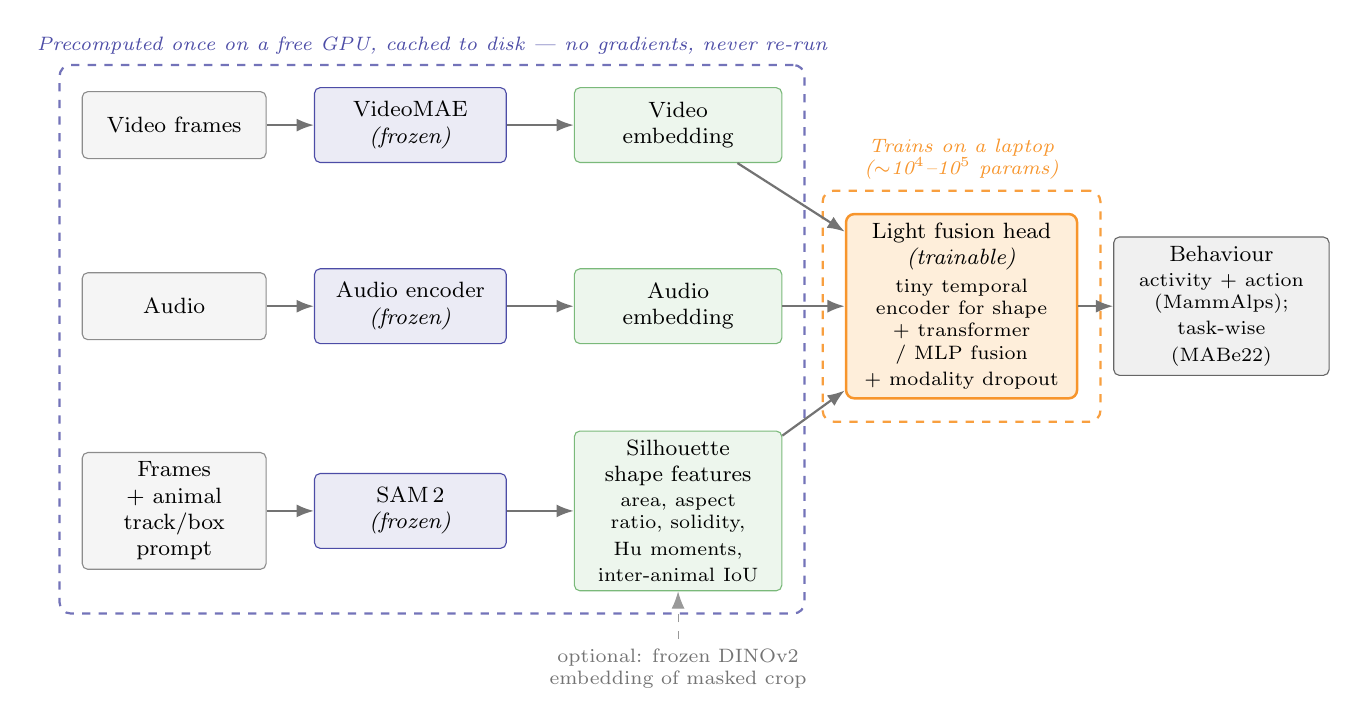
\begin{tikzpicture}[
  font=\footnotesize,
  >={Latex[length=2.2mm]},
  inp/.style   ={rectangle, rounded corners=2pt, draw=black!45, fill=black!4,  align=center, text width=2.1cm, minimum height=0.85cm},
  frozen/.style={rectangle, rounded corners=2pt, draw=NavyBlue!70, fill=NavyBlue!8, align=center, text width=2.2cm, minimum height=0.95cm},
  feat/.style  ={rectangle, rounded corners=2pt, draw=ForestGreen!60, fill=ForestGreen!8, align=center, text width=2.4cm, minimum height=0.95cm},
  train/.style ={rectangle, rounded corners=3pt, draw=BurntOrange!85, line width=0.9pt, fill=BurntOrange!12, align=center, text width=2.7cm, minimum height=1.6cm},
  result/.style={rectangle, rounded corners=2pt, draw=black!60, fill=black!6, align=center, text width=2.5cm, minimum height=1.2cm},
  flow/.style  ={->, draw=black!55, thick},
]
% inputs
\node[inp] (vidin) at (0, 2.3)  {Video frames};
\node[inp] (audin) at (0, 0.0)  {Audio};
\node[inp] (mskin) at (0,-2.6)  {Frames\\+ animal\\track/box prompt};
% frozen encoders
\node[frozen] (vmae) at (3.0, 2.3)  {VideoMAE\\\textit{(frozen)}};
\node[frozen] (aenc) at (3.0, 0.0)  {Audio encoder\\\textit{(frozen)}};
\node[frozen] (sam)  at (3.0,-2.6)  {SAM\,2\\\textit{(frozen)}};
% cached features
\node[feat] (vemb) at (6.4, 2.3)  {Video\\embedding};
\node[feat] (aemb) at (6.4, 0.0)  {Audio\\embedding};
\node[feat] (shp)  at (6.4,-2.6)  {Silhouette shape features\\[1pt]\scriptsize area, aspect ratio, solidity,\\ Hu moments, inter-animal IoU};
% trainable fusion
\node[train] (fuse) at (10.0, 0.0) {Light fusion head\\\textit{(trainable)}\\[2pt]\scriptsize tiny temporal encoder for shape\\$+$ transformer / MLP fusion\\$+$ modality dropout};
% output
\node[result] (out) at (13.3, 0.0) {Behaviour\\[1pt]\scriptsize activity $+$ action (MammAlps);\\ task-wise (MABe22)};
% arrows
\draw[flow] (vidin) -- (vmae);  \draw[flow] (audin) -- (aenc);  \draw[flow] (mskin) -- (sam);
\draw[flow] (vmae) -- (vemb);   \draw[flow] (aenc) -- (aemb);   \draw[flow] (sam)  -- (shp);
\draw[flow] (vemb) -- (fuse);   \draw[flow] (aemb) -- (fuse);   \draw[flow] (shp)  -- (fuse);
\draw[flow] (fuse) -- (out);
% optional DINOv2
\node[align=center, text=black!55, font=\scriptsize] (dino) at (6.4,-4.6) {optional: frozen DINOv2\\embedding of masked crop};
\draw[->, draw=black!40, dashed] (dino) -- (shp);
% zones
\begin{scope}[on background layer]
  \node[draw=NavyBlue!55, dashed, thick, rounded corners,
        fit=(vidin)(mskin)(vmae)(sam)(vemb)(shp), inner sep=8pt,
        label={[text=NavyBlue!70, font=\scriptsize\itshape, align=center]above:Precomputed once on a free GPU, cached to disk --- no gradients, never re-run}] {};
  \node[draw=BurntOrange!75, dashed, thick, rounded corners,
        fit=(fuse), inner sep=8pt,
        label={[text=BurntOrange!85, font=\scriptsize\itshape, align=center]above:Trains on a laptop\\($\sim$10$^{4}$--10$^{5}$ params)}] {};
\end{scope}
\end{tikzpicture}
\caption{Initial architecture. Heavy encoders (blue) are run once and cached; only the small fusion head (orange) is trained. The mask branch defaults to cheap hand-crafted shape descriptors---roughly the footprint of pose keypoints---with a heavier DINOv2 embedding held in reserve.}
\label{fig:arch}
\end{figure}

\paragraph{Training and protocol.} Only the head trains, on cached features, on an M4 Pro (PyTorch MPS). Use official splits with a fixed seed; report \emph{mean $\pm$ std over several seeds}, since on datasets this small a $+0.02$ mAP can be noise. Keep the head capacity identical across conditions so any gain reflects \emph{information}, not parameters; an optional control feeds a blanked/scrambled mask (same parameters, no real shape) to confirm the silhouette is doing the work. Hierarchical heads (activity + action) on MammAlps; task-wise heads on MABe22; balanced sampling and per-class reporting throughout.

% ---------------------------------------------------------------------
\section{Novelty}
% ---------------------------------------------------------------------
The contribution is \emph{not} ``fuse audio + video + mask and tabulate it''---that alone would be a thin engineering exercise. It is the first treatment of the animal \emph{silhouette shape as a learned, fused modality} for behaviour, with explicit inter-animal contact geometry and a background-robustness test. Each near neighbour is distinct:
\begin{itemize}
  \item \textbf{MammAlps scene maps}~\cite{mammalps}: a \emph{background} map per viewpoint (no animal shape); shown not to help. We test \emph{foreground} shape.
  \item \textbf{PanAf-FGBG}~\cite{panaf}: SAM\,2 masks used to \emph{erase} the animal and study the background; gains come from background, not silhouette. We keep the silhouette as a positive signal---and use their result as motivation, since shape is the representation that discards the background they show models over-rely on.
  \item \textbf{MAROON}~\cite{maroon}: mask-guided action recognition exists, but masks form background-removed cutouts (Mask-R-CNN, not SAM), with no pose and no treatment of shape as its own fused stream.
  \item \textbf{LookAgain}~\cite{lookagain}: keypoint$\leftrightarrow$video fusion using raw video, no masks; its per-behaviour asymmetry motivates a dedicated shape stream for contact behaviours.
\end{itemize}

% ---------------------------------------------------------------------
\section{Expected results}
% ---------------------------------------------------------------------
The core deliverable is an ablation ladder plus a per-behaviour analysis (Table~\ref{tab:expected}). The aggregate bar to beat is the audio-sized gain ($\approx +0.02$ mAP); the sharper test is per-class.

\begin{table}[h]
\centering
\begin{tabular}{@{}lcl@{}}
\toprule
Configuration & Class-avg mAP & Reading \\
\midrule
Video only            & $\approx 0.45^{\dagger}$ & baseline to reproduce \\
\quad $+$ audio        & $\approx 0.47^{\dagger}$ & audio adds $\approx +0.02$ (the bar) \\
\quad $+$ mask (shape) & \textbf{target $\gtrsim$ audio} & RQ1/RQ2: does shape match/beat the audio gain? \\
Video $+$ audio $+$ mask & \textbf{?} & RQ1: does shape add \emph{on top of} audio? \\
\bottomrule
\end{tabular}
\caption{Anticipated pattern (not measured results). $^{\dagger}$Figures reported by MammAlps~\cite{mammalps}, read partly from figures; to be reproduced from released features before any comparison is claimed.}
\label{tab:expected}
\end{table}

\noindent\textbf{What each outcome means.}
\begin{itemize}
  \item \emph{Strong positive:} video+mask beats video-only by at least the audio gain, \emph{or} a clear per-class win ($\sim+0.03$--$0.05$ AP) on contact/posture behaviours (chasing, mounting, Oral--Genital Contact). Headline: shape helps where background maps did not, and for the ``right'' (background-free) reasons---supported by the robustness test (RQ4).
  \item \emph{Publishable either way:} any consistent per-class gain on contact classes, with mask-dropout robustness demonstrated.
  \item \emph{Clean negative:} if shape does not help (or only where pose already suffices, echoing LookAgain), that is itself a tidy, citable result---MammAlps already showed background maps don't help; ``foreground shape doesn't either, and here is why'' closes the question and directly informs whether a shape stream is worth adding to PoseR.
\end{itemize}

% ---------------------------------------------------------------------
\section{Feasibility}
% ---------------------------------------------------------------------
None of the heavy models is ever in the training loop: each is run once on Kaggle's free GPU and its outputs cached, so they are a bounded, one-time preprocessing cost rather than a per-step one. The trained head sees only a handful of cached vectors, so it is tiny and re-runs in minutes on a laptop---keeping the experiment in line with PoseR's lightness philosophy, whose real target is cheap \emph{deployment} over long footage. If shape proves useful and cheap inference later matters, there are ready routes (keep the hand-crafted branch, drop the mask via the modality-dropout design, or distil), treated here as future work. The one genuinely heavy step is the single SAM pass to generate masks; this is batched, cached, and gated by a checkpoint around week~5 to reassess if MammAlps night/infrared footage makes masking too slow or noisy---at which point the headline experiment moves to the clean MABe22 setting and MammAlps becomes a stress test.

% ---------------------------------------------------------------------
\section*{Indicative timeline}
% ---------------------------------------------------------------------
\noindent
\begin{tabular}{@{}rl@{}}
\textbf{Wk 1} & Read core papers; reproduce MammAlps video / video+audio baselines from cached features.\\
\textbf{Wk 2} & SAM\,2 on Kaggle; generate + cache masks for MABe22 (clean case).\\
\textbf{Wk 3} & Shape-feature + inter-animal overlap extractor; sanity checks.\\
\textbf{Wk 4} & Light fusion head + modality dropout; video vs video+mask on MABe22 contact classes.\\
\textbf{Wk 5} & Cache SAM masks for MammAlps; QC mask quality; go/no-go decision.\\
\textbf{Wk 6} & Full MammAlps ablation: video $\to$ +mask $\to$ +audio $\to$ +audio+mask.\\
\textbf{Wk 7} & Missing-modality robustness; per-class \& background-shift analysis.\\
\textbf{Wk 8} & Write-up; figures; package cached-feature pipeline + code.\\
\end{tabular}

% ---------------------------------------------------------------------
% NOTE: author lists / titles below are seeded and must be verified
% against each source before submission (arXiv IDs are confirmed live).
% ---------------------------------------------------------------------
\begin{thebibliography}{99}
\bibitem{mammalps} V.~Gabeff et al. \emph{MammAlps: A multi-view, multimodal benchmark for wildlife behaviour recognition.} CVPR, 2025. arXiv:2503.18223.
\bibitem{panaf} O.~Brookes et al. \emph{The PanAf-FGBG Dataset: Understanding the Impact of Backgrounds in Wildlife Behaviour Recognition.} CVPR, 2025. arXiv:2502.21201.
\bibitem{maroon} F.~Schindler, V.~Steinhage, S.~T.~S.~van Beeck Calkoen, and M.~Heurich. \emph{Action Detection for Wildlife Monitoring with Camera Traps Based on Segmentation with Filtering of Tracklets (SWIFT) and Mask-Guided Action Recognition (MAROON).} Applied Sciences, 14(2):514, 2024. doi:10.3390/app14020514.
\bibitem{lookagain} W.~Li, J.~Ke, Y.~Wang, C.~Li, A.~Wu. \emph{Learning When to Look: On-Demand Keypoint--Video Fusion for Animal Behavior Analysis.} 2026. arXiv:2603.07279.
\bibitem{sam2} N.~Ravi et al. \emph{SAM\,2: Segment Anything in Images and Videos.} ICLR, 2025. arXiv:2408.00714.
\bibitem{mabe22} J.~J.~Sun et al. \emph{The MABe22 Benchmark: Learning multi-agent and multi-species behavior representations.} ICML, 2023. arXiv:2207.10553.
\bibitem{dinov2} M.~Oquab et al. \emph{DINOv2: Learning Robust Visual Features without Supervision.} TMLR, 2024. arXiv:2304.07193.
\bibitem{actionmae} S.~Woo et al. \emph{Towards Good Practices for Missing Modality Robust Action Recognition (ActionMAE).} AAAI, 2023. arXiv:2211.13916.
\bibitem{stgcn} S.~Yan, Y.~Xiong, D.~Lin. \emph{Spatial Temporal Graph Convolutional Networks for Skeleton-Based Action Recognition.} AAAI, 2018.
\bibitem{poser} P.~N.~Mullen, B.~Bowlby, H.~C.~Armstrong, A.~Gray, and M.~F.~Zwart. \emph{PoseR: a deep learning toolbox for classifying animal behaviour.} Open Biology, 16(1):250322, 2026. doi:10.1098/rsob.250322.
\end{thebibliography}

\end{document}